%========================================================================================
% TU Dortmund, Informatik Lehrstuhl VII
%========================================================================================

\chapter{Spring-Embedder}
\label{Kapitel 3}
%


\begin{figure}[t]
	\centering
	\subfigure[rote Knoten sind die Stahlkugeln verbunden mit Federn]
	{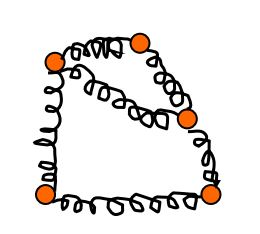
\includegraphics[scale=0.6]{bilder/graphfederfirst}\label{fig_graphfederfirst}
	}
	\hspace{1.0cm}%
	\subfigure[die Federn verschieben die Knoten]
	{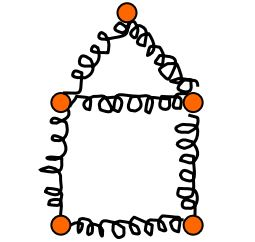
\includegraphics[scale=0.6]{bilder/graphfedersecond}\label{fig_graphfedersecond}
	}
	\hspace{1.0cm}%
	\subfigure[darstellung als Graph]
	{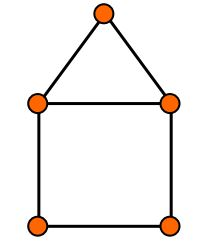
\includegraphics[scale=0.6]{bilder/graphfederthird}\label{fig_graphfederthird}
	}
	\\
	\caption[Darstellung als Stahlkugeln und Federn eines Graphen]{Darstellung als Stahlkugeln und Federn eines Graphen}
	\label{fig_testbild2}
\end{figure}
In diesem Kapitel werden die Grundlagen des Spring-Algorithmus erklärt, der im Kapitel 4 dazu verwendet wird um eine MetroMap ähnliche Darstellung des Höchstspannungsnetzes zu erhalten. Es geht um die Verwendung dieser Algorithmen und das grundsätzliche Vorgehen. Ebenso werden auf Unterschiede zwischen den meist verwendeten Spring-Embedder eingegangen.

\section{Spring-Embedder - allgemein}
\label{Kapitel_3_-_Unterkapitel_2}

Auf Kräfte basierte Algorithmen gehören zu den flexibelsten Methoden zur Berechnung eines simplen Layouts für ungerichtete Graphen. Diese Algorithmen, auch Spring-Embedder genannt, beruhen nur auf der zugrunde liegenden Struktur des Graphen. Zeichnungen des Graphen die aus diesen Algorithmen resultieren, neigen dazu sehr ästhetisch und symmetrisch zu sein. Zudem liefern sie meist einen überschneidungsfreie Darstellung des Graphen sofern dieser planar ist.[Spring Embedders and Force Directed GraphDrawing Algorithms] \\

Die folgenden Ausführungen stammen aus dem Buch \grqq Software-Practice and Experience, VOL. 21(1 1), 1129-1164"(November 1991).

 
Das Problem der Darstellung basiert auf der Platzierung der Kanten sowie
Knoten um eine möglichst ästhetische Zeichnung des
Graphen zu erhalten, die gut lesbar und verständlich ist. Die grundlegenden Kriterien für eine ästhetischen Zeichnung eines Graphen sind:
\begin{enumerate}
	\item die Knoten sollten gleichmäßig verteilt werden
	\item minimale Überschneidung der Kanten
	\item einheitliche Länge der Kanten
	\item möglichst symmetrisch
	\item alles soll sich innerhalb der Fläche befinden[Graph Drawing by Force-directed Placement].
\end{enumerate}   

Das heißt es ist leicht möglich die wichtigen Informationen des Graphen anhand einer visuellen Darstellung zu erhalten. Dazu gehören unter anderem die Erkennung von Verbindungen zwischen Knoten oder deren Lage. Dies ist vor allem wichtig bei einer MetroMap wo es darum geht schnell herauszufinden wie es möglich ist von einem Punkt zu einem anderen zu kommen. Um dies zu erreichen gibt es verschiedenste Ansätze. Diese müssen auf dem verwendeten Graphen anwendbar sein, sollten jedoch auch simpel und effizient sein.\\


Im Folgenden wird es um eine Erweiterung eines Verfahrens gehen, welches auf Grundlage des von Peter D. Eades entwickelten Algorithmus aus dem Jahre 1984 basiert. Er erklärt seine Metapher wie folgt:

\begin{quote}
	The basic idea is as follows. To embed [lay out] a graph we replace the
	vertices by steel rings and replace each edge with a spring to form a
	mechanical system . . . The vertices are placed in some initial layout and
	let go so that the spring forces on the rings move the system to a minimal
	energy state.
\end{quote}

Es geht demnach um ein Modell, indem die Knoten durch Stahlringe und die Kanten durch Federn repräsentiert werden. Durch die Federn wirken anschließend Kräfte auf die Kugeln ein, wodurch sich diese verschieben. Die Kugeln sollten jedoch vorher zufällig verteilt werden damit es mit diesem Vorgang zu einer besseren Lösung kommt. 
Das Verschieben der Kugeln durch die Federn passiert solange bis es zu einem sogenannten minimal-energy-state kommt. Das bedeutet, dass die Federn und Kugeln in einer Position befinden, indem die einwirkenden Kräfte der Federn keine Bewegung der Kugeln mehr zulassen. Dies ist meist erreicht sobald die Federn ihre optimale Länge erreicht haben, sie demnach keine weitere Kraft mehr auf die Kugeln wirken können. Es kommt jedoch nicht immer dazu. Es kann passieren, dass sich von zwei Federn, die noch nicht ihre optimale Länge haben, durch die Konstellation der Knoten ihre wirkende Kraft gegeneinander auflöst.\\

Die wirkenden Kräfte der Federn können nach belieben gewählt werden und müssen dabei nicht dem Hookeschem Gesetz entsprechen. Das hookesche Gesetz beschreibt die elastische Verformung von Festkörpern, wenn deren Verformung proportional zur einwirkenden Belastung ist[Wikipedia]. Es können demnach beliebige Definitionen, der wirkenden Kräfte der Federn, benutzt werden um ein gewünschtes Ergebnis zu erreichen. Ein weiterer Unterschied zur physikalischen Realität ist die Anwendung der Kraft auf die Knoten. Es können beliebige Knoten gewählt und auf diese, die gewünschte Kraft angewendet werden. Im Folgenden werden anziehende Kräfte zwischen jedem Knotenpaar, welches durch eine Kanten verbunden ist, angewendet. Abstoßende Kräfte wirken zwischen jedem Knoten, die nicht miteinander verbunden sind, demnach ebenso nicht durch eine Feder modelliert wurden. Das sind die Freiheiten des Verfahrens im Vergleich zur Realität. \\

Ein weiteres sehr ähnliches Verfahren, welches auf dem von Eades beruht ist der Algorithmus von Kamada und Kawai. Sie modellierten den Graphen ebenfalls als ein System von Federn, jedoch, im Vergleich zu Eades, hielten sich sie sich an das Hockesche Gesetz und versuchten dieses mit mehreren Differentialgleichungen zu lösen um ein verbessertes Layout zu erhalten. Eades hielt es für sehr wichtig, dass verbundene Knoten nah zueinander gezeichnet werden, demnach hat er ausschließlich anziehende Kräfte zwischen verbundenen Knoten berechnet. Kamada und Kawai haben hingegen ein weiteres Konzept eingefügt, welches auch anziehende Kräfte zwischen nicht verbundenen Knoten berechnet. Diese Kräfte sind proportional zur Länge des kürzesten Pfades der beiden Knoten. Das Problem der Zeichnung eines Graphen sahen Kamada und Kawai als das Vorgehen zur Reduzierung der noch zu wirkenden Kräfte der Federn in dem Graphen. Ist ein Zustand erreicht in dem die Summe der wirkenden Kräfte der Federn zum Tiefpunkt gekommen ist, so sind die Positionen und Abstände der Knoten nahe zu optimal gewählt. Sie definierten die komplette Energie des Graphen als: 

\begin{align}
	\sum_{\leq i < j\leq |V|}k_{p_{v_{i}}p_{v_{j}}}(|p_{v_{i}}-p_{v_{j}}|-l_{v_{i}v_{j}})^{2}
\end{align}

wobei $p_{v_{i}}$ die Position des Ringes oder Knotens $v_{i}$ ist, $k_{p_{v_{i}}p_{v_{j}}}$ ist die Feder-Konstante zwischen den Positionen $p_{v_{i}}$ und $p_{v_{j}}$ und $l_{v_{i}v_{j}}$ ist der optimale Abstand der beiden Knoten $v_{i}$ und $v_{j}$. Diese Energie wird reduziert durch das Lösen von Differentialgleichungen eines Knotens zur Findung einer besseren Position mit einer geringeren Menge an Energie im System. Die Positionierung der Knoten findet so lange statt, bis eine gegebene Grenze erreicht wurde. Ein wesentlicher Unterschied im Vergleich zu Eades Algorithmus ist, dass pro Iteration immer nur ein Knoten bewegt wird. \\





\section{Spring-Embedder - Vorgehen}
\label{Kapitel_3_-_Unterkapitel_2}
%
\begin{figure}[t]
	\centering
	{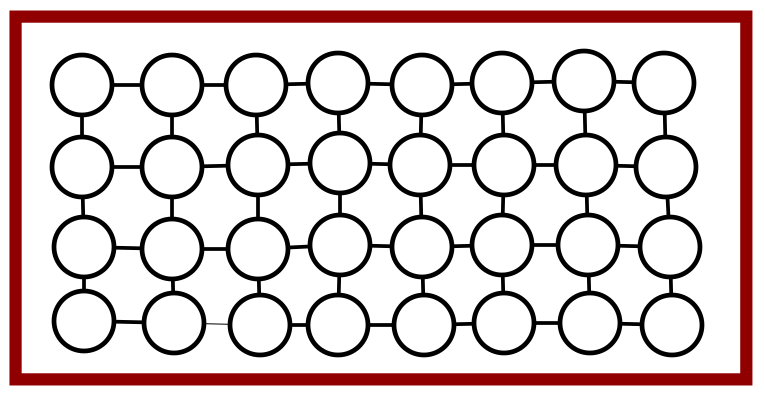
\includegraphics[scale=0.5]{bilder/grenzeundperfekteverteilung}\label{fig_grenzeundperfekteverteilung}
	}\\
	\caption[Eine Beispielhafte Abbildung der Knoten mit einer nahezu perfekten Verteilung]{Eine Beispielhafte Abbildung der Knoten mit einer nahezu perfekten Verteilung}
	\label{fig_grenzeundperfekteverteilung}
\end{figure}
 Die optimale Länge der Kanten $k$, die als Federn modelliert werden, wird durch die Anzahl der Knoten sowie der zur Verfügung stehender Fläche $A$ bestimmt:

\begin{align}
	k =
	C\sqrt{A / |V|}
\end{align}

\begin{align}
	A =
	W * L.
\end{align}

$W$ ist die Weite und $L$ die Länge der zugrunde liegenden Oberfläche, auf der, der Graph gezeichnet wird. Es ist wichtig zu wissen wie diese Maße sind um eine bessere Verteilung der Knoten zu ermöglichen. Da die bessere Verteilung der Knoten zu einem ästhetischen Graphen führt wird versucht die Oberfläche optimal zu nutzen. Wie weit Knoten voneinander entfernt sein sollten, wird demnach durch die Anzahl der Knoten und der Oberfläche bestimmt. Besonders wichtig ist es, dass die Knoten nicht zu nah aber auch nicht zu weit voneinander entfernt gezeichnet werden, denn beides führt zu einer Verschlechterung der Attraktivität des Graphen. $k = C\sqrt{A / |V|}$ führt dazu, dass sich die Knoten $|V|$ weit genug voneinander entfernt befinden um die Fläche gut zu nutzen und ebenso nah genug sind um die Ästhetik der Zeichnung zu bewahren. Die optimale Distanz $k$ gibt somit auch die freie Fläche um einen Knoten an. Je weiter die momentane Distanz von der optimalen Distanz zwischen den Knoten abweicht, desto größer sollte ihr Einfluss auf das Layout werden. Die Neuausrichtung der Knoten passiert drastischer, wenn die Knoten noch zu weit von ihrer optimalen Distanz von einander entfernt sind und verringert sich sobald die Knoten näher an ihre optimale Distanz zu einander kommen. Dabei macht es keinen Unterschied ob die Knoten zu nah oder zu weit von einander entfernt sind. In der Abbildung 3.x wird die perfekte Verteilung der Knoten dargestellt. Die rote Umrandung gibt den Rand des Bildes an. Die Knoten sind dort alle symmetrisch verteilt mit einem optimalen Abstand zu einander. Die Knoten haben auf dieser Abbildung auch eine orthogonale Lage. Der Algorithmus führt jedoch nicht immer zu einer orthogonalen Positionierung.  \\
 
Die Konstante $C$ sollte experimentell gewählt werden, denn die Struktur eines Graphen kann stark variieren. Um dennoch in der Lage zu sein auf diese Schwankungen reagieren zu können kann die Konstante $C > 1$ beliebig vergrößert werden um einen größeren optimalen Abstand zu erhalten oder bei $C < 1$ die Größe des Abstandes verringern. \\

Bildet die bisherige Platzierung der Kanten und Knoten einen planaren Graphen, so wird die neue Platzierung in fast allen Fällen auch planar sein. Ein Graph ist planar wenn sich keine Kanten überschneiden, diese Eigenschaft ist besonders gewollt um den resultierenden Graphen noch übersichtlicher zu gestalten. \\


\begin{algorithm}[t]
	\centering
	\caption[Spring-Algorithmus]{Spring-Algorithmus} \label{algo_1}
	\begin{algorithmic}[1]
		\REQUIRE \begin{math} G:= (V,E) \end{math}
		\ENSURE \begin{math} G:= (V,E) \end{math}
		\FOR{\begin{math}i:=1 \leq iterations \end{math}}
		\FOR{\begin{math}v_{i} \in V\end{math}}
		\STATE $d_{v_{i}} := 0;$
		\FOR{(\begin{math}v_{j} \in V\end{math})}
		\IF{$v_{i}\neq v_{j}$}
		\STATE $\Delta := p_{v_{i}} - p_{v_{j}};$
		\STATE $d_{v_{i}} := d_{v_{i}} + (\Delta / |\Delta|) \cdot f^{r}_{v_{i},v_{j}}(|\Delta|));$
		\ENDIF
		\ENDFOR
		\ENDFOR
		\newline
		\FOR{\begin{math}e_{v_{i},v_{j}} \in E\end{math}}
		\STATE $\Delta := p_{v_{i}} - p_{v_{j}};$
		\STATE $d_{v_{i}} := d_{v_{i}} - (\Delta / |\Delta|) \cdot f^{a}_{v_{i},v_{j}}(|\Delta|));$
		\STATE $d_{v_{j}} := d_{v_{j}} + (\Delta / |\Delta|) \cdot f^{a}_{v_{i},v_{j}}(|\Delta|));$
		\ENDFOR
		\newline
		\FOR{\begin{math}v_{i} \in V\end{math}}
		\STATE $p_{v_{i}} := p_{v_{i}} + ( d_{v_{i}}/ |d_{v_{i}}|) \cdot min ( d_{v_{i}}, t );$
		\STATE $p_{v_{i}}^{x} := min(W/2, max(-W/2, p_{v_{i}}^{x}));$
		\STATE $p_{v_{i}}^{y} := min(L/2, max(-L/2, p_{v_{i}}^{y}))$
		\ENDFOR
		\STATE $t:= cool(t)$
		\ENDFOR
	\end{algorithmic}
\end{algorithm}

Die Ein- sowie Ausgabe des in 3.1 vorgestellten Algorithmus, ist ein Graph $G:= (V,E)$, der bereits eine gewisse Positionierung der Knoten hat. Dieser kann sofern er noch keine hat, eine zufällige Positionierung der Knoten vor Beginn des Algorithmus erhalten, was den Algorithmus sogar noch effektiver macht, da sich dadurch einige Probleme vermeiden lassen, was mit reellen Graphen öfter der Fall ist. Auf die möglich auftretenden Probleme werden in diesem Kapitel auch noch eingegangen. Die meisten Herausforderungen sind die lokalen Minima und die dadurch entstehenden Ausreißer. \\

Zwischen jedem Knotenpaar $v_{i},v_{j} \in V$ wird eine abstoßende Kraft \begin{math} f^{r}_{v_{i},v_{j}}  \end{math} berechnet.   Alle benachbarten Knoten erhalten eine anziehende Kraft \begin{math} f^{a}_{v_{i},v_{j}} \end{math}. Zwei Knoten \begin{math} v_{i},v_{j} \in V \end{math}sind benachbart wenn \begin{math} e_{v_{i},v_{j}} \in E \end{math} ist. Das führt dazu, dass verbundene Knoten näher zusammen gezeichnet werden, während sie noch immer einen gewissen Abstand zueinander haben. Der Algorithmus geht dabei in drei Schritten vor:

\begin{enumerate}
	\item zwischen jedem Knotenpaar die abstoßende Kraft berechnen
	\item benachbarten Knoten eine anziehende Kraft zuweisen
	\item jeden Knoten seiner neuen Kraft nach bewegen.
\end{enumerate} 
Diese drei Schritte werden werden so oft wiederholt bis keine weitere Bewegung mehr stattfindet. Die Anzahl der Iterationen können auch fest gewählt werden, um eine Obergrenze einzuhalten. Eine weitere Möglichkeit ist die $cool(t)$ Funktion zur Regulierung der Bewegungsmöglichkeiten der Knoten. Die genaue Wirkung und Vorgehensweise der Funktion wird am Ende des Kapitels noch erläutert.

Die Funktionen \begin{math} f^{a}_{v_{i},v_{j}} \end{math} und \begin{math} f^{r}_{v_{i},v_{j}} \end{math} sind wie folgt definiert:


\begin{align}
	f^{a}_{v_{i},v_{j}} (x) =
	x^{2}/k
\end{align}

\begin{align}
	f^{r}_{v_{i},v_{j}} (x) =
	-k^{2}/x.
\end{align}


\begin{figure}[t]
	\centering
	\subfigure[anziehende Kraft $f^{a}$ zwischen dem dritten und vierten Knoten]
	{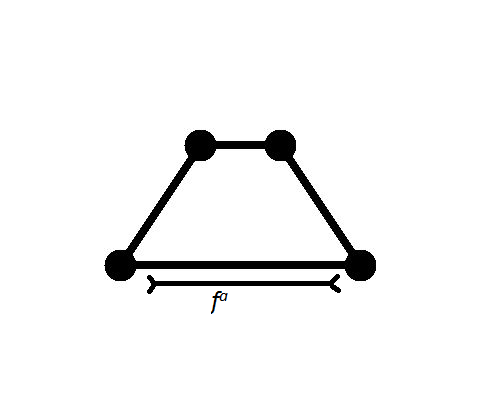
\includegraphics[scale=0.5]{bilder/kraftfa}\label{fig_kraftfa}
	}
	\hspace{1.0cm}%
	\subfigure[abstoßende Kraft $f^{r}$ zwischen dem ersten und vierten Knoten]
	{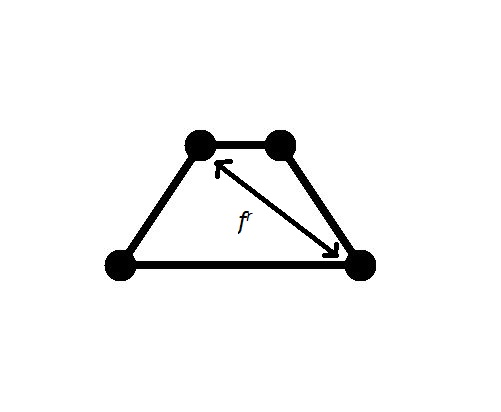
\includegraphics[scale=0.5]{bilder/kraftfr}\label{fig_kraftfr}
	}
	\hspace{1.0cm}%
	\subfigure[die wirkenden Kräfte lösen sich auf]
	{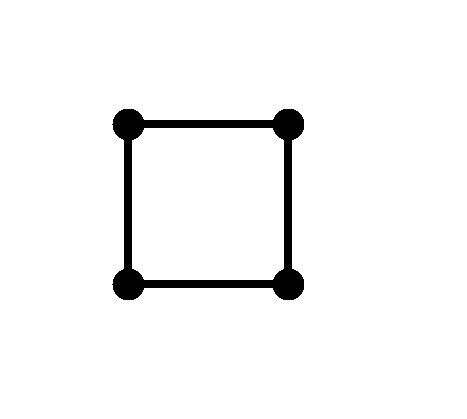
\includegraphics[scale=0.5]{bilder/standardgraph}\label{fig_standardgraph}
	}
	\\
	\caption[Wirkende Kräfte im Graphen]{Wirkende Kräfte im Graphen}
	\label{fig_testbild2}
\end{figure} 

\begin{figure}[t]
	\centering
	{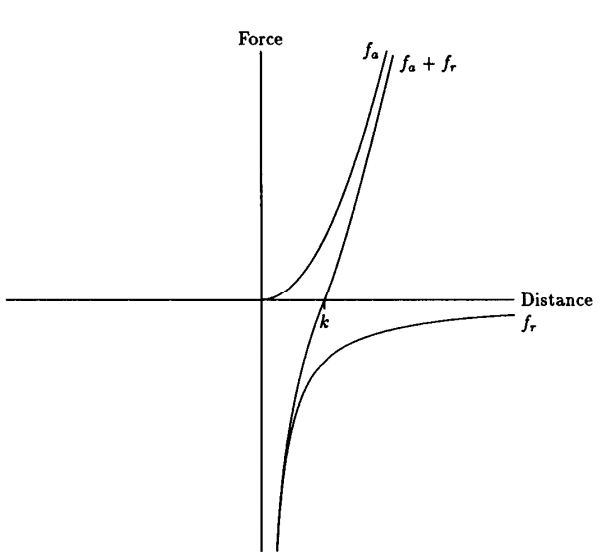
\includegraphics[scale=0.7]{bilder/forcevsdistance}\label{fig_forcevsdistance}
	}\\
	\caption[Verhältnis der Kräfte zueinander und deren Einluss auf die optimale Distanz]{Verhältnis der Kräfte zueinander und deren Einluss auf die optimale Distanz}
	\label{fig_forcevsdistance}
\end{figure}

In der Abbildung 3.x ist das Verhältnis zwischen den Kräften und der optimalen Distanz $k$ abgebildet. Die x-Achse stellt die Distanz dar und die y-Achse die Wirkung der Kräfte $f^{a}_{v_{i},v_{j}}$, $f^{r}_{v_{i},v_{j}}$. Die Summe der beiden Kräfte wird mit der Funktion $f^{a}_{v_{i},v_{j}}$ + $f^{r}_{v_{i},v_{j}}$ dargestellt. Wenn die Summe der beiden Kräfte null erreicht, ist dies die optimale Distanz $k$. Das passiert auf der x-Achse, sofern sich die abstoßende Kraft und die anziehende Kraft gegenseitig auflösen. \\

Die beiden Funktionen wurden dabei experimentell gewählt. Sie ergaben sich bei der Implementierung und ähnelten dem hookeschen Gesetz. Dabei ergaben sich auch andere Funktionen wie:

\begin{align}
f^{a}_{v_{i},v_{j}} (x) =
x/k
\end{align}

\begin{align}
f^{r}_{v_{i},v_{j}} (x) =
-k/x.
\end{align}

\begin{figure}[t]
	\centering
	\subfigure[Ausgangsgraph mit den Knoten A, B, C, D]
	{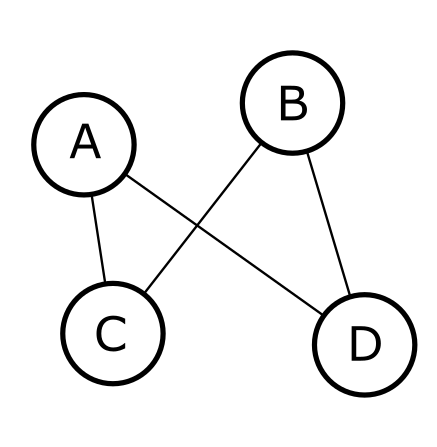
\includegraphics[scale=0.5]{bilder/abcdminima1}\label{fig_abcdminima1}
	}
	\hspace{1.0cm}%
	\subfigure[Positionierung nach der Anwendung des Algorithmus]
	{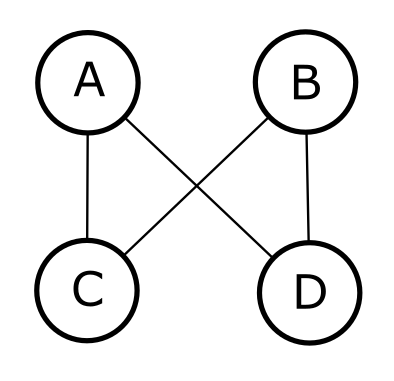
\includegraphics[scale=0.5]{bilder/abcdminima3}\label{fig_abcdminima3}
	}
	\hspace{1.0cm}%
	\subfigure[Bestmögliche Positionierung der Knoten]
	{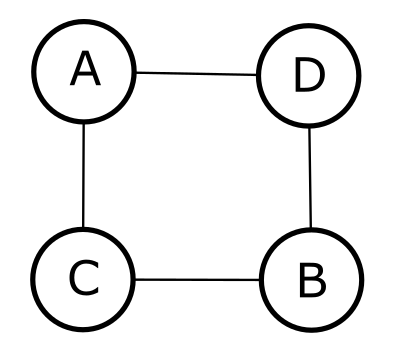
\includegraphics[scale=0.5]{bilder/abcdminima2}\label{fig_abcdminima2}
	}
	\\
	\caption[Lokales Minima-Problem]{Lokales Minima-Problem}
	\label{fig_testbild2}
\end{figure}

\begin{figure}[t]
	\centering
	\subfigure[Positionierung vor Anwendung des Algorithmus]
	{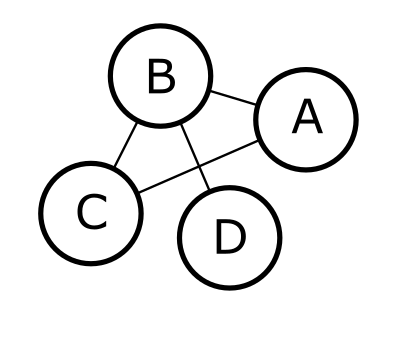
\includegraphics[scale=0.5]{bilder/abcdminima6}\label{fig_abcdminima6}
	}
	\hspace{1.0cm}%
	\subfigure[Anwendung des Algorithmus mit der Entstehung des Ausreißer D]
	{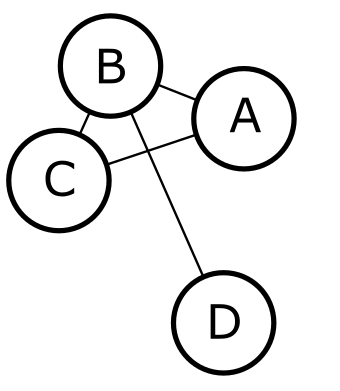
\includegraphics[scale=0.5]{bilder/abcdminima5}\label{fig_abcdminima5}
	}
	\hspace{1.0cm}%
	\subfigure[Mögliche Positionierung der Knoten ohne Bildung eines Ausreißer]
	{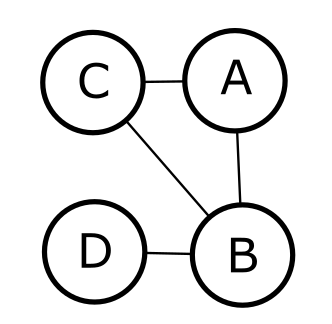
\includegraphics[scale=0.5]{bilder/abcdminima4}\label{fig_abcdminima4}
	}
	\\
	\caption[Bildung von Ausreißer]{Bildung von Ausreißer}
	\label{fig_testbild2}
\end{figure}

\begin{figure}[t]
	\centering
	\subfigure[Mögliche Positionierung nach der Anwendung des Algorithmus]
	{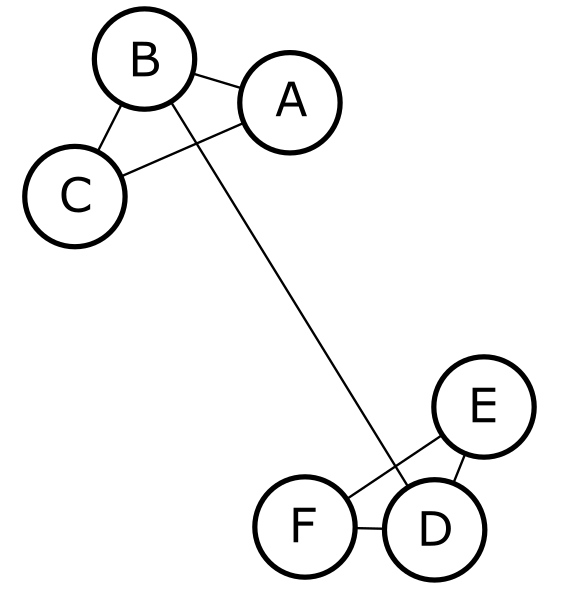
\includegraphics[scale=0.4]{bilder/ballenbildung}\label{fig_ballenbildung}
	}
	\hspace{1.0cm}%
	\subfigure[Eine bessere Positionierung der Knoten ohne die Bildung von Ballen]
	{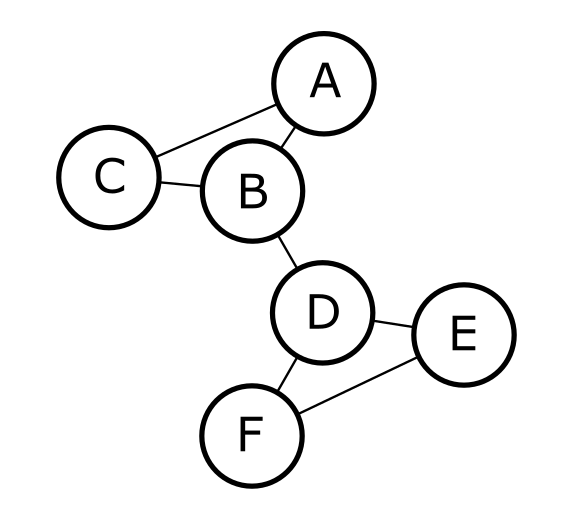
\includegraphics[scale=0.4]{bilder/ballenbildung2}\label{fig_ballenbildung2}
	}
	\\
	\caption[Resultat von Ballenbildung und dessen Auswirkung auf das Layout]{Resultat von Ballenbildung und dessen Auswirkung auf das Layout}
	\label{fig_testbild2}
\end{figure}
 
 Diese schienen auch das Problem zu lösen, lieferten aber bei komplexeren Graphen weitaus schlechtere Layouts. Das lag daran, dass sie nicht in der Lage waren ein sogenanntes lokales Minima zu überwinden. Ein lokales Minima tritt auf, wenn die initiale Positionierung eines Knotens sich in den Weg eines anderen Knotens stellt und sich dieser deswegen in eine eigentlich schlechtere Position bringt. Dieser Knoten müsste seine schlechte Position dadurch verbessern, dass er erst durch eine weitaus schlechtere Positionierung geht um anschließend eine bessere Position zu erhalten. Dieser Vorgang wird auch als $hill climbing$ bezeichnet. Da die Knoten durch Kräfte bewegt werden, die stets eine bessere Position anstreben, dabei aber nicht wissen, wie sich die anderen Knoten in Zukunft platzieren werden, ist ein direktes Vorgehen gegen dieses Problem mit diesem Ansatz nicht möglich. Die Funktionen $f^{a}_{v_{i},v_{j}}$, $f^{r}_{v_{i},v_{j}}$ ergaben weitaus öfter den Fall, dass Knoten in einem lokalen Minima feststecken und sich dabei nicht mehr in eine bessere Position bringen konnten. Je größer die wirkenden Kräfte gewählt werden, desto wahrscheinlicher ist es, dass sich ein Knoten in einem Schritt an einen anderen vorbei bewegt und somit ein lokales Minima verhindert. In der Abbildung 3.x wird das lokale Minima Problem anhand eines kleinem Beispiel veranschaulicht. Vor der Anwendung des Algorithmus ist die Positionierung der Knoten wie in 3.x(a). Wird der Algorithmus nun angewendet verteilen sich die Knoten wie in der Abbildung 3.x(b). Sie können demnach nicht das lokale Minima überkommen. In 3.x(c) ist eine mögliche perfekte Darstellung der Knoten zu sehen. Die Knoten B und D oder aber die Knoten A und C müssten die Position komplett tauschen, was jedoch voraussetzt, dass erst einmal eine schlechtere Positionierung gewählt werden muss um zu dieser Darstellung zu kommen. Der Algorithmus wird demnach auch nach beliebig vielen Iterationen immer in diesem Minima stecken bleiben und niemals zur besseren Darstellung in 3.x(c) übergehen können. \\
 
 Durch dieses Problem treten auch die sogenannten Ausreißer auf. Das sind Knoten die sich in eine besonders schlechte Position gebracht haben, dadurch, dass sie in einem lokalen Minima gefangen sind. Diese Position wird meist immer weiter verschlechtert und führt zu einer sehr unschönen Zeichnung, die geprägt wurde von einigen dieser Ausreißer. In der Abbildung 3.x(a) ist ein Graph zu sehen, welcher mit Anwendung des Algorithmus zur Bildung eines Ausreißers führt. Der Knoten D liegt bereits vor Ausführung des Algorithmus nicht optimal. Eine optimale und planare Darstellung des Graphen ist in der Abbildung 3.x(c) zu sehen. Es ist also möglich den Graphen planar und kompakt zu zeichnen, indem die Knoten überschneidungsfrei und alle die optimale Distanz zueinander haben. In der Abbildung 3.x(b) entsteht durch die Anwendung des Algorithmus der Ausreißer D. Dieser Knoten wird durch die abstoßenden Kräfte von den Knoten A, B und C weiter nach außen gedrückt und nur die anziehende Kraft zwischen B und D ist nicht stark genug um diesen näher zu halten. Dieser Knoten wird sich nicht mehr bewegen, sobald die Summe der abstoßenden Kräfte und der anziehenden Kraft gleich null ist und sie sich in einem Gleichgewicht befinden. Durch die ungünstige Verteilung der Knoten zu Beginn des Algorithmus und die besonderen Kanten zwischen ihnen, kommt es letztendlich zur Bildung eines Ausreißers. \\ 
 
 Ein ähnliches Problem des Algorithmus, was auch zu einem lokalen Minima führt, ist die Bildung von einzelnen vielen Knoten an verschiedenen Punkten, die meist nur durch wenige Kanten miteinander verbunden sind. Diese Ballen von Knoten entstehen wie die Ausreißer, nur dass es nicht einzelne Knoten sind sondern eine Sammlung von Mehreren. In der Abbildung 3.x(a) ist dieses Problem aufgetreten. Wenn die Knoten zu Beginn des Algorithmus bereits ähnlich, wie in dieser Abbildung zu sehen ist, liegen. So ist sehr wahrscheinlich, dass sich dort ein lokales Minima bildet. Dieses Minima wird dadurch definiert, dass sich die Knoten nicht mehr in eine optimale Lösung bewegen können, da sie sich vorher in eine schlechtere Position bringen müssten. Die Knoten A und C sowie E und F stoßen die Knoten B und D nach außen. Die Knoten B und D können durch diese abstoßende Kraft nicht zur ihrer optimalen Distanz gebracht werden, da die Kraft dafür nicht ausreichend ist. Die anziehenden Kräfte von A,C,E und F auf die Knoten B und D tragen dazu auch verstärkend bei. Diese Positionierung der Knoten würde auch nach beliebig vielen Iterationen nicht in ein optimales Layout resultieren, denn die Kräfte haben sich bereits ausbalanciert, was keine weitere Bewegung mehr zulässt. Eine optimale Lösung bei diesem Graphen, wäre ähnlich wie in der Abbildung 3.x(b). Die Knoten B und D haben ihre lokales Minima beschränkend durch die Knoten A, C, E, F überwunden, was zu einem deutlich besseren Layout führt.  \\
 
 
Zur Bewegung der Knoten wurde ein Vektor $d_{v_{i}}$ eingeführt, dieser gibt an in welcher Richtung der Knoten $v_{i}$ bewegt wird. Während der Vektor $p_{v_{i}}$ auf die momentane Position des Knoten $v_{i}$ zeigt. Der Vektor $\Delta$ ist die Differenz zwischen $p_{v_{i}}$ und $p_{v_{j}}$, der Richtungsvektor von $v_{i}$ nach $v_{j}$. Die Variable $iterations$ gibt die Anzahl der Durchläufe an. \\

Bei jedem neuen Durchlauf wird der Vektor  $d_{v}$  eines jeden Knotens $v$ auf null gesetzt. Dies geschieht in Zeile 3 des Algorithmus 3.1. Mit zwei For-Schleifen wird jede Knotenkombination durchgegangen und anschließend wird die abstoßende Kraft $f^{r}_{v_{i},v_{j}}$ mithilfe der Länge des $\Delta$ Vektors berechnet. Der $\Delta$ Vektor ist nichts anderes als der Abstand zwischen den zwei Knoten, dieser wird gebraucht um die Kraft anhand des bereits vorhandenen Abstandes zu regulieren. Sind zwei Knoten $v_{i}$, $v_{i}$ bereits sehr weit entfernt, so wird die berechnete Kraft in der Funktion $f^{r}_{v_{i},v_{j}}$ durch die Eingabe von $\Delta$ schwächer ausfallen. Anschließend wird die berechnete Kraft mit dem Einheitsvektor multipliziert und auf den Bewegungsvektor schließlich addiert. Dadurch drücken sich die Knoten direkt voneinander weg. \\

In den Zeilen 11-15 geschieht der zweite Schritt des Algorithmus, die Berechnung der anziehenden Kraft zwischen den benachbarten Knoten. Dazu wird jede Kante einmal mit Hilfe einer For-Schleife durchgegangen und wie bei der Berechnung der abstoßenden Kraft muss auch der Abstand zwischen den beiden Knoten $v_{i}$, $v_{i}$ für die Funktion $f^{a}_{v_{i},v_{j}}$ vorher berechnet werden, um festzustellen, ob die Knoten bereits die optimale Distanz zu einander haben. Ist dies der Fall, so wird berechnete anziehende Kraft deutlich schwächer ausfallen, als bei Knoten die noch zu weit von einander entfernt sind. Anschließend wird auch hier der Bewegungsvektor mit dem Ergebnis der Berechnung aktualisiert. \\

Dadurch dass jeder Knoten nun mehrmals eine Aktualisierung seines Bewegungsvektor erhalten hat, durch den Einfluss aller Knoten untereinander, ist dieser nun sehr genau bestimmt worden und die Knoten können sich in seine angegebene Richtung bewegen. Im letzten Schritt des Algorithmus, demnach Zeile 16-20, werden die Knoten nun in Richtung ihres Bewegungsvektors bewegt. Die Zeilen 18 und 19 dienen dabei, dass der Knoten während der Bewegung nicht die Grenzen des Bildes verlässt. \\


Die Variable $t$ ermöglicht es, am Anfang viel Bewegung der Knoten zuzulassen und dies immer weiter einzuschränken, damit mit der Graph mit jeder Iteration feiner wird. Die Funktion $cool(t)$ regelt dabei wie weit sich jeder Knoten in der nächsten Iteration maximal bewegen darf. $t$ könnte zum Beispiel bei der Länge des Bildes starten und sich nach jeder Iteration um ein Zehntel mit $cool(t)$ kürzen. Nach zehn Iterationen wären dadurch keine weiteren Bewegungen der Knoten mehr möglich. Die Implementierung dieser Funktion zeigte jedoch keinen sichtbaren Unterschied zur manuellen Regulierung der Iterationen. Dadurch wurde diese Funktion im Folgenden Kapitel ebenfalls nicht benutzt. Anstatt dessen, wird der Algorithmus durch eine verschiedene Anzahl an Iterationen getestet. 

